\documentclass{article}
\usepackage{graphicx}
\title{Gravitas}
\author{}
\date{}
\begin{document}
\maketitle
Welcome to Gravitas\footnote{Weight and seriousness in Latin}, a LiquidFun game!

\section{Build}
To build Gravitas on your platform, you need to provide \verb|libglut.a|, \verb|libglui.a| and \verb|libliquidfun.a| in \verb|lib| directory. Then run \verb|make| and you'll get the executable file in \verb|bin/main|.
\section{Play}
In this game, the player can control the direction of the gravity.
The goal is to transfer some water to a given exit.

\begin{center}
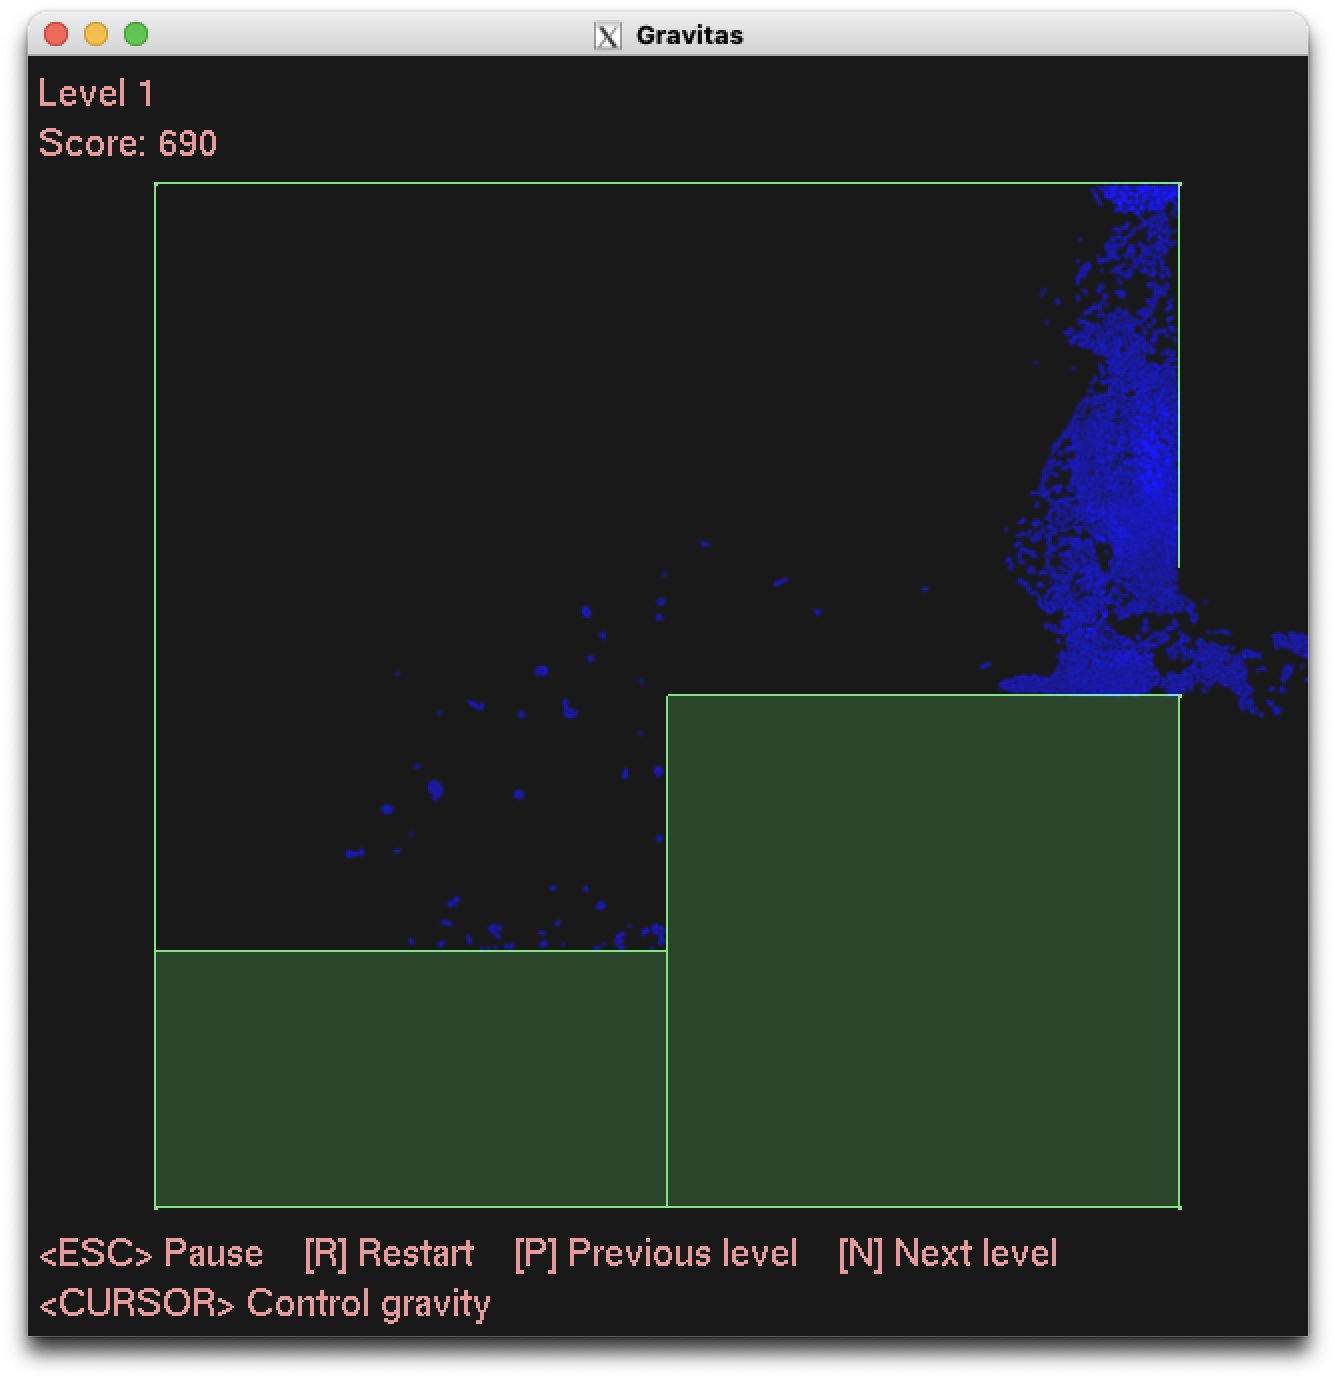
\includegraphics[width=200px]{Level1.png}
\end{center}
In Level 1, we'll learn how to control the gravity.

\begin{center}
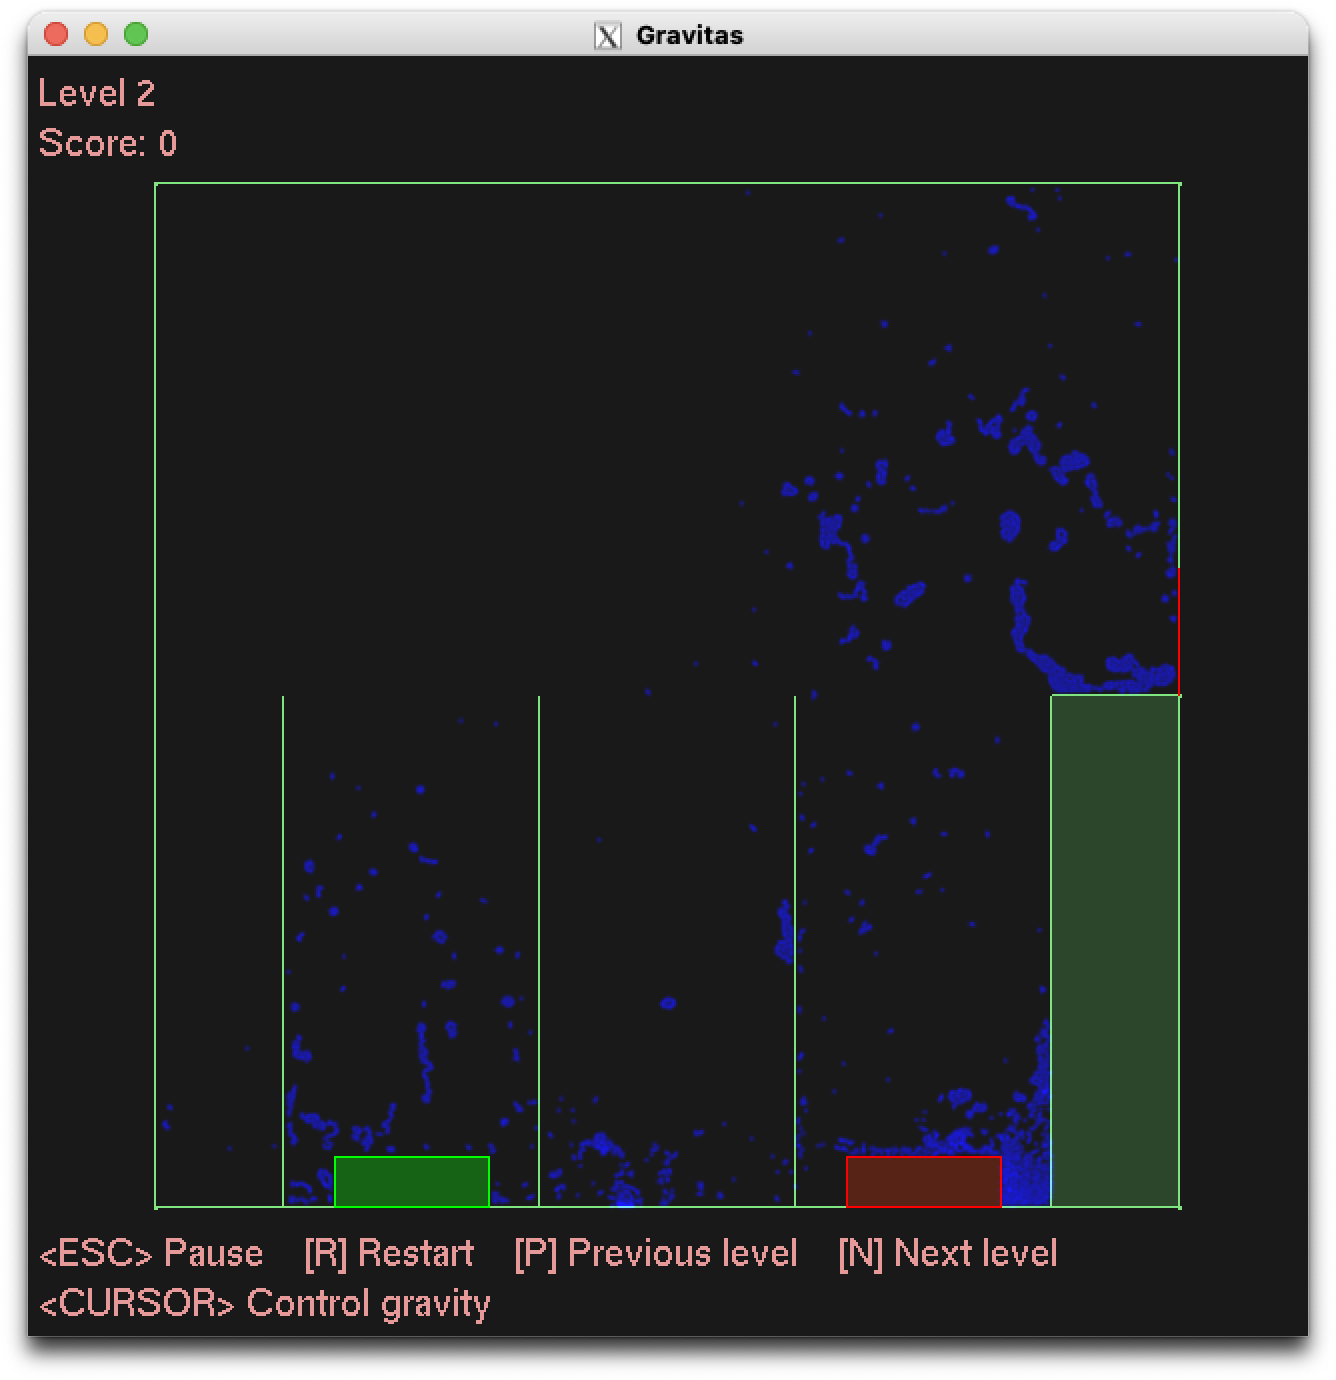
\includegraphics[width=200px]{Level2.png}
\end{center}
In Level 2, a new mechanism --- trigger is introduced.
You need to put some weight on the trigger to open the door.

\begin{center}
    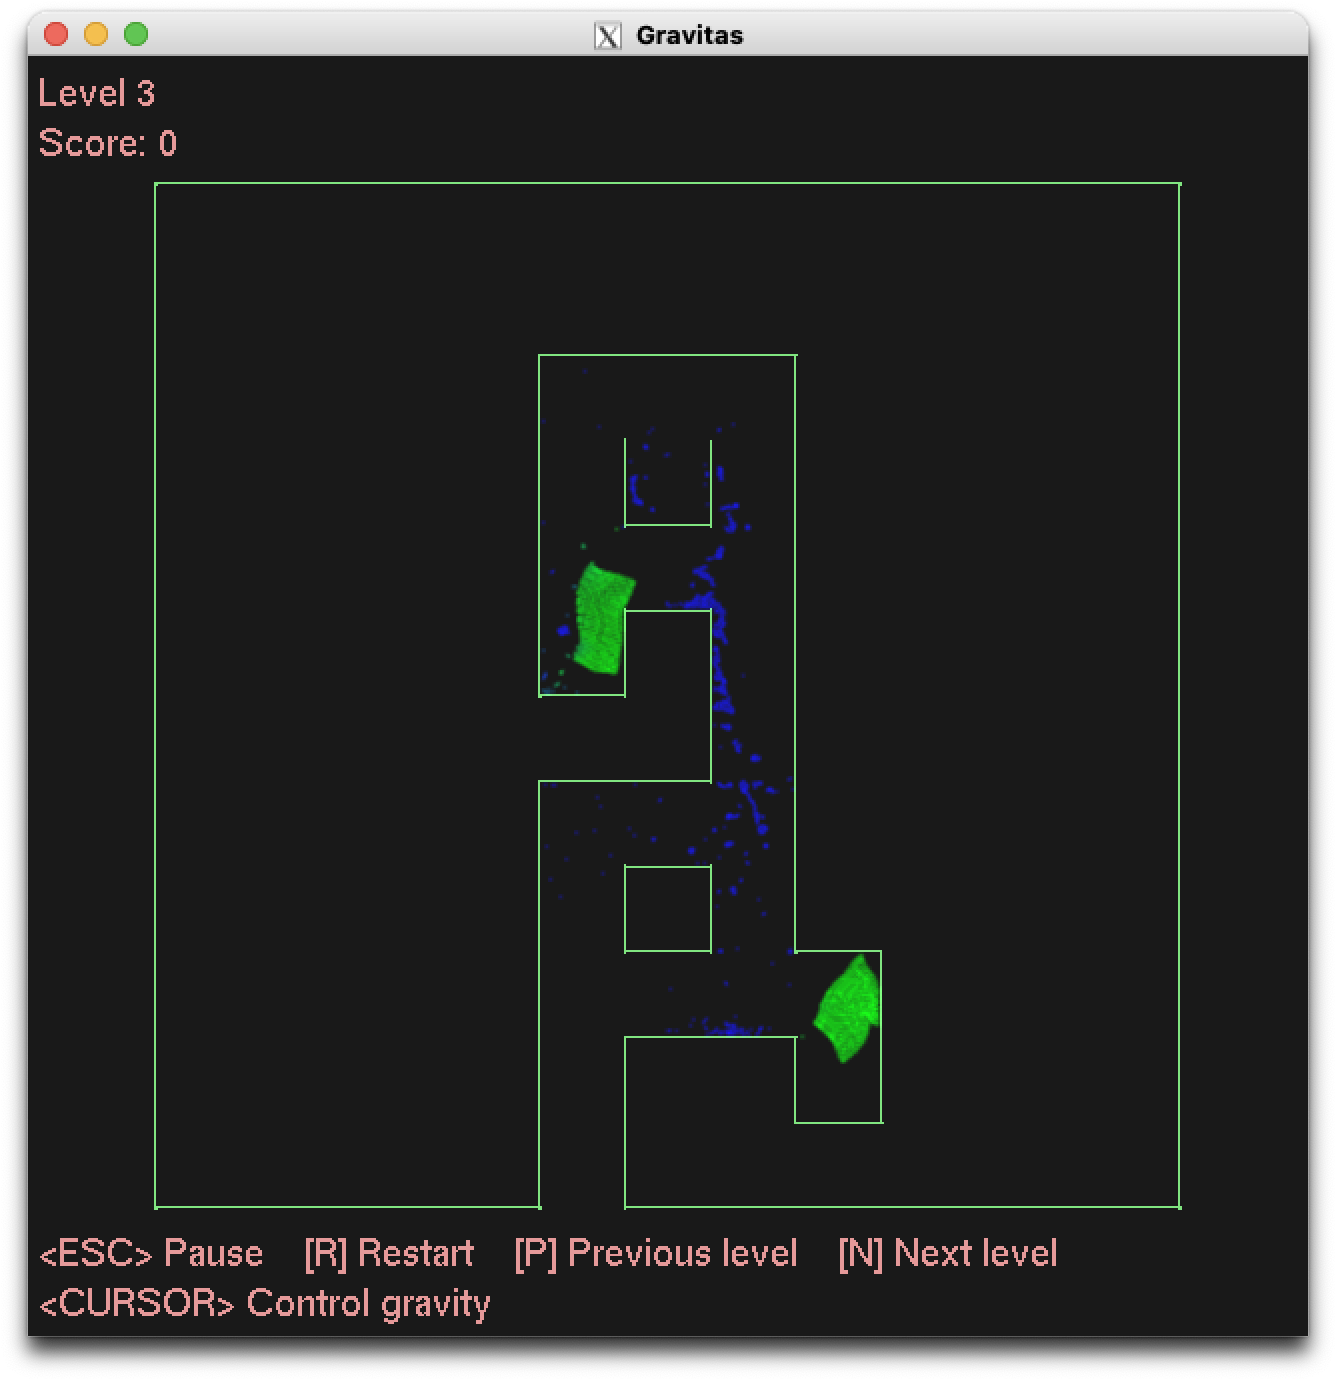
\includegraphics[width=200px]{Level3.png}
    \end{center}
In Level 3, poisonous elastic block crashed the party.
If poisonous water gets into the exit, you lose.
Since it's elastic, be careful to make use of the gravity to prevent it from escaping!

\begin{center}
    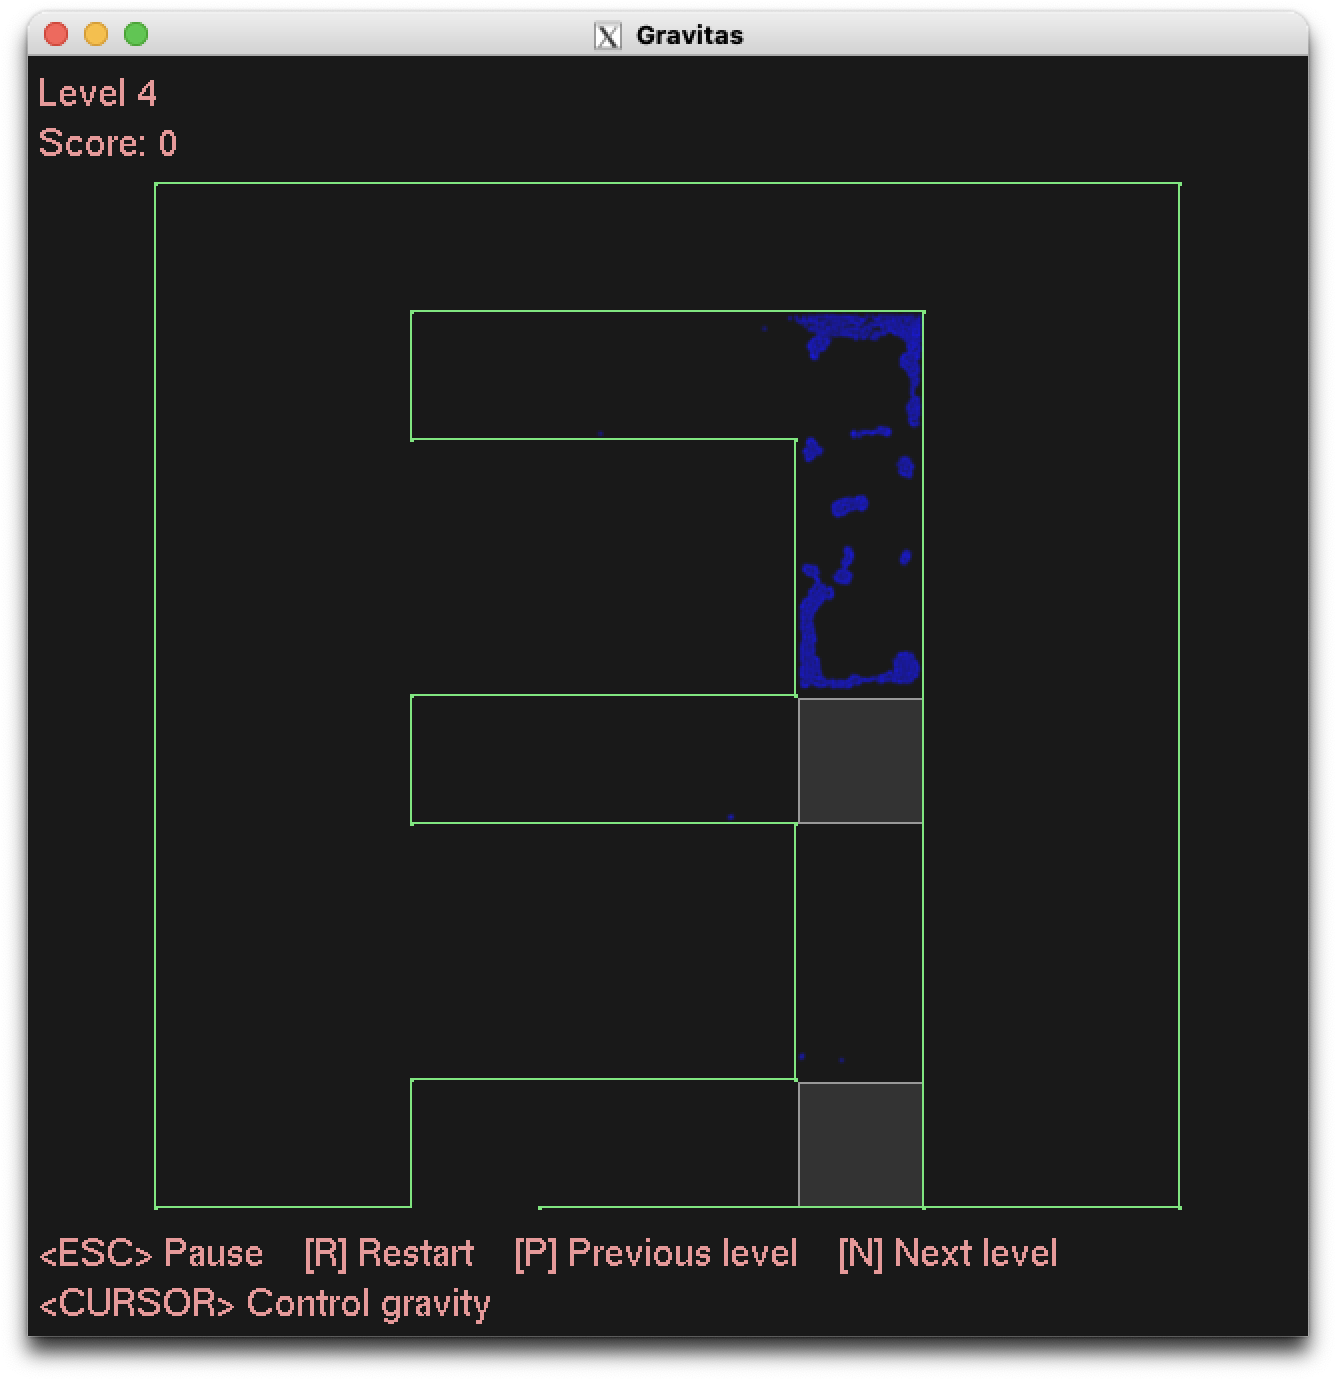
\includegraphics[width=200px]{Level4.png}
    \end{center}
In Level 4, we'll meet a magic power that connects two blocks together!
It's kind of difficult (it confused two of my friends!), try if you could solve the puzzle!

\section{Test}
To run the unit tests:
\begin{enumerate}
    \item Build the project.
    \item Cd to the \verb|testcase| directory, and run \verb|make|.
    \item Run the executable file.
\end{enumerate}

\section{Design}
\subsection{Overall}
I've implemented 4 levels now. I've implemented the required two effects, water-flow effect and elastic object collision effect. The latter is demonstrated in Level 3, while the former is everywhere in the game.
The game is now basically playable with a simple GUI and saving support.

Since the API of LiquidFun is too old and does not conform to OOP design principles, I made some encapsulation of the original API, for example, you can see in my code a customized class \verb|Water| is used to create liquid.
In this way I can reuse the code of creating water, and at the same time improve readability.

I found design patterns useful in managing the development process. For example, I applied Singleton Pattern in \verb|SaveManager| to manage the saving process of the game. 
Factory Method Pattern is used to control the instantiation of levels.

\subsection{Framework}
The game is based on the TestBed framework of LiquidFun.
\verb|Main.cpp| is responsible for using glui to create windows and process keyboard input.
\verb|Render.cpp| is responsible for rendering the graphics using OpenGL.
\verb|Level.cpp| defines a base class for a level.

\subsection{SaveManager}
\verb|SaveManager| is a singleton class that manages the saving progress of the game.

During the construction of the only instance, file \verb|save.dat| is loaded. If it already exists, it reads the current progress from the file and records it. Otherwise, it creates the file.
During the destruction of the only instance (that means the program is exiting), the current level is written to \verb|save.dat|.

By using the singleton pattern, we manages the saving progress easily, safely and universally.
Since there is only one instance, we do not need to care about the ownership of the instance.
And we also don't need to worry about when to read and write the save file, since that's done by the construction and destruction of the instance when the program starts and ends.

\subsection{LevelManager}
\verb|LevelManager| manages the statistics of the current game.

It stores a threshold for winning the game and the current score.
We use \verb|leaking| function to tell the level manager that some liquid is leaking out of the screen. Then it either increments or decrements the score depending on the type of the leaking liquid.

Functions \verb|increment|, \verb|decrement| could be used to manage the score manually. Function \verb|getScore|, \verb|didWin| and \verb|didLose| could be used to check the current game status. Function \verb|showScore| could be used to draw the score on the screen.

\subsection{Level}
Class \verb|Level| inherits \verb|b2ContactListener| to serve as a particle contact listener.

Member variable \verb|id| stores the id of the level.

Member variable \verb|destructionListener| stores an instance of the auxiliary class \verb|DestructionListener|, which binds to a \verb|LevelManager| object. When a liquid particle is destructed, the destruction listener is called and then it forwards the information to the level manager to update the score.

Function \verb|drawTitle| prints the current level and tips for control the game.

Callback function \verb|KeyboardSpecial| is called when a special key (here, the cursor keys) is pressed.
We set the direction of the gravity on the basis of the key pressed.
By the way, to make it more flexible, we set the intensity of the gravity somewhere else, not here.
Hence when we'd like to change the intensity of the gravity, we do not need to modify this function.

Callback function \verb|Step| is called every 1/60 second.
It firstly calls LiquidFun to simulate the movement and calls the particle system to destroy particles that go out of the screen, then calls the level manager to show the score and if won, calls the save manager to save the progress.

In the concrete \verb|Level| subclasses, we creates the game elements in the constructor, like the borders, the ground, the water and the mechanics like triggers and doors. 
We also set the level complete threshold here.

\subsection{LevelFactory}
To manage the creation process of the levels, we applies the factory pattern.

Abstract class \verb|LevelFactory| defines a pure virtual function \verb|create| that returns a \verb|unique_ptr<Level>|.

In \verb|Levels.h|, we stores some instances of each concrete level factory.
In this way, we separate the \verb|Level| class from the creation process of \verb|Level| instances.

\subsection{Water}
Since water is everywhere in the game, we extracts the creating process of Water using raw LiquidFun API to this class.

The constructor of \verb|Water| takes various kinds of parameters, like the type of the water, the flags of the water and so on.
To avoid unnecessary efforts, default parameters are used here to provide default behavior of the water.

We also provide a static function \verb|getColor| to decide the color of specific kind of water.
In this way, when we want to change the color of one kind of water, we just need to modify one place instead of everywhere this kind of water exists.

\subsection{Trigger \& Door}
These two mechanics uses the principle of encapsulation to avoid unexpected modification.

For example, since \verb|Door| only provides the interface \verb|open|, you cannot close it after it is opened. In this way we could make sure that a door stays open once it has been opened.
\verb|Trigger| only provides the interface \verb|trigger|. This increments the trigger count monotonously, so that once a trigger is triggered, it remains triggered.

\end{document}